\documentclass{article}

\usepackage[T1]{fontenc}
\usepackage{cite}
\usepackage{graphicx} 
\usepackage{caption}    
\usepackage{subcaption} 
\usepackage{booktabs}
\usepackage{array}
\usepackage{siunitx}
\usepackage{float}
\usepackage{tabularx}
\usepackage{indentfirst}
\usepackage{xcolor}

\renewcommand{\arraystretch}{1.2}
\setlength{\tabcolsep}{6pt}

\title{Capacitively-Coupled Chopper Instrumentation Amplifier for Linear Hall Effect Sensor \\[1ex] \large IEEE SSCS Chipathon 2026}
\author{Team Chop}
\date{\today}

\setcounter{secnumdepth}{0}

\begin{document}

\maketitle

\newpage

\tableofcontents

\newpage

\section{Project Information}

\begin{center}
\begin{tabular}{|c c|} 
 \hline
 Project Name & CCIA for Linear Hall Effect Sensor \\
 \hline
 Team Members & alang \\ 
 \hline
 Review Date &  \\
 \hline
 Review Version &  \\
 \hline
 Track & B \\
 \hline
\end{tabular}
\end{center}

\newpage

\section{Design Objective}

The aim of this project is to design and characterize a monolithic magnetic sensing system based on the Hall Effect. 
If tapeout is completed, the specifications of the sensor and readout circuit will be characterized individually.

The target specifications for the magnetic sensing system are shown in Table~\ref{tab:system_specs}. 
See the Appendix for the full working specification documents for all blocks. 

\begin{table}[H]
    \centering
    \begin{tabular}{|c c|}
        \hline
        \textbf{Specification} & \textbf{Value} \\
        \hline
        Maximum Offset & \SI{100}{\micro\tesla} \\
        \hline
        Area & \SI{0.25}{\milli\meter\squared} \\
        \hline
        Resolution & \SI{100}{\micro\tesla}\textsubscript{rms} \\
        \hline
        Input Range & $\pm$\SI{100}{\milli\tesla} \\
        \hline
        Bandwidth & \SI{10}{\kilo\hertz} \\
        \hline
        Supply Voltage & \SI{3.3}{\volt} \\
        \hline
        Supply Current & \SI{2}{\milli\ampere} \\
        \hline
        Temperature Range & \SIrange{-40}{125}{\degreeCelsius} \\
        \hline
        Clock Frequency & \SI{100}{\kilo\hertz} \\
        \hline
        Output Common-Mode Voltage & \SI{1}{\volt} \\
        \hline
    \end{tabular}
    \caption{System Specifications}
    \label{tab:system_specs}
\end{table}

The motivation for this project in the context of the Chipathon program is to provide reusable IP to the open-source silicon community.
Priority will be given to designing a simple system that can be well characterized as opposed to a novel system.
Overall, if the tapeout is successful, future designers would be able to reuse and customize both the sensor design and
the readout circuit for their specific application. In any case, future Chipathon participants will be able to learn from the 
successes and failures of the project. 

\newpage

\section{System Overview}

A block diagram of the system is shown in Fig.~\ref{fig:block_diagram}. 

\begin{figure}[htbp]
    \centering
    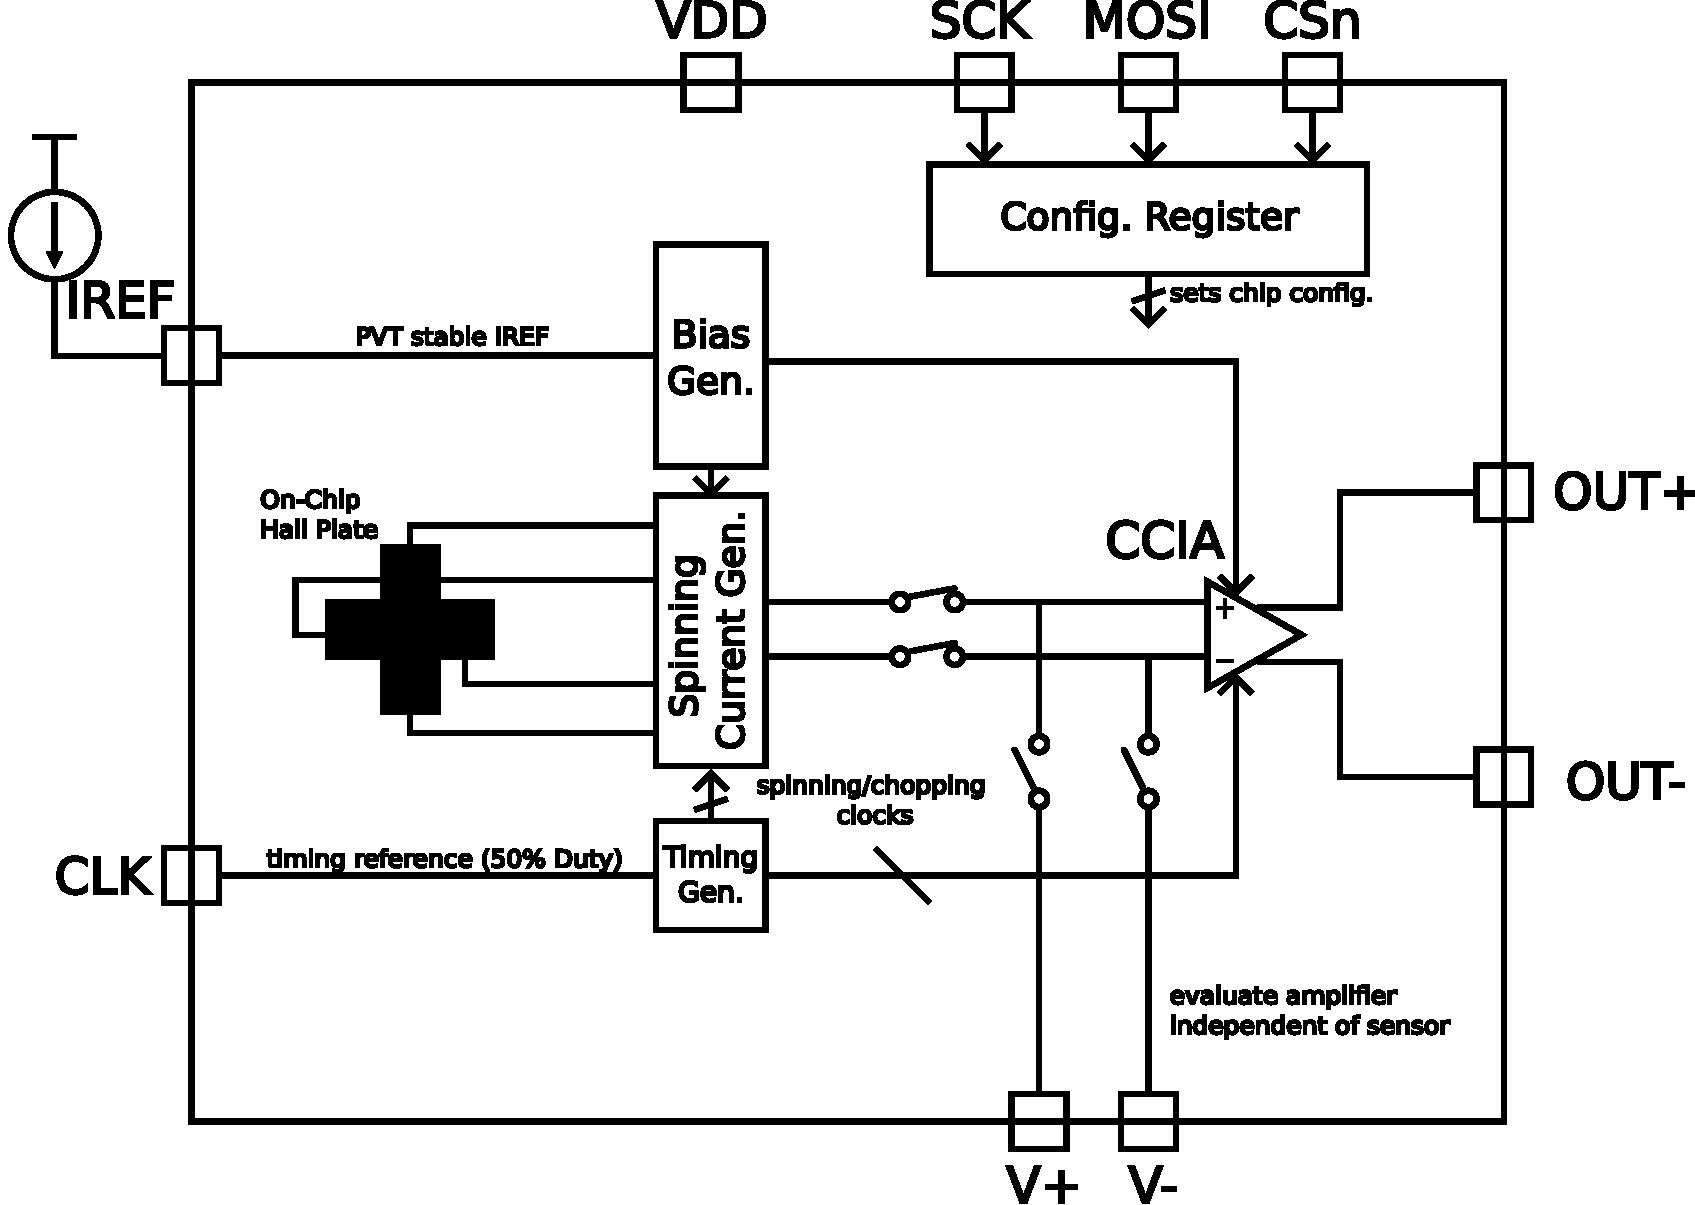
\includegraphics[width=\linewidth]{figs/chip_block_diagram.pdf}
    \caption{Block diagram of the proposed architecture.}
    \label{fig:block_diagram}
\end{figure}

In the diagram, an on-chip horizontal Hall plate converts an incoming magnetic
field (perpendicular to plane of chip) into a small voltage that is amplified by the instrumentation amplifier (IA)
prior to being driven to the DUT output pins (OUT+/OUT-). The entire design operates from 
a single supply. Aside from the SPI configuration interface (only used during idle periods), 
the entire design operates in a single synchronous clock domain derived from the external clock signal (CLK).
Two additional pins are used as analog debug pins (V+/V-). Based on the system configuration, these pins will used
to probe various points within the design to enable individual characterization of the sensor and IA.

A full pinout table of the design is given in Table~\ref{tab:pinout}.

\begin{table}[H]
    \centering
    \begin{tabularx}{\linewidth}{l l X}
        \toprule

        \multicolumn{3}{l}{\textbf{Analog Pins}} \\
        \midrule
        IREF   & Analog & Current reference \\
        OUT+   & Analog & (+) Output \\
        OUT-   & Analog & (-) Output \\
        VTP+   & Analog & (+) Test Point \\
        VTP-   & Analog & (-) Test Point \\
        \midrule

        \multicolumn{3}{l}{\textbf{Digital Pins}} \\
        \midrule
        SCK    & Digital Input & SPI configuration clock \\
        MOSI   & Digital Input & SPI configuration data input \\
        CSn    & Digital Input & SPI chip select \\
        CLK    & Digital Input & Chopping/spinning clock reference \\
        \midrule

        \multicolumn{3}{l}{\textbf{Supply Pins}} \\
        \midrule
        VDD    & Power & Supply input \\
        VSS    & Power & Ground (shared with other Chipathon blocks) \\
        \bottomrule
    \end{tabularx}
    \caption{Project I/O description.}
    \label{tab:pinout}
\end{table}

\newpage

\section{Schematic Summary}

This section describes the schematic-level operation of each part of the design. For each block, 
both behavioral and transistor-level models are described, including motivation for key design 
decisions. For all blocks, the transistor-level sizing is subject to change during the verification
process.

\subsection{On-Chip Hall Plate}

\begin{itemize}
    \item{Purpose}
    \item{Inputs and Outputs}
    \item{Sub-sheets}
    \item{Behavioral Model}
    \item{Design Methodology}
    \item{Transistor-Level Implementation}
\end{itemize}

\subsection{Bias Generation}

\begin{itemize}
    \item{Purpose}
    \item{Inputs and Outputs}
    \item{Sub-sheets}
    \item{Behavioral Model}
    \item{Design Methodology}
    \item{Transistor-Level Implementation}
\end{itemize}

\subsection{Spinning Current Generation}

\begin{itemize}
    \item{Purpose}
    \item{Inputs and Outputs}
    \item{Sub-sheets}
    \item{Behavioral Model}
    \item{Design Methodology}
    \item{Transistor-Level Implementation}
\end{itemize}

\subsection{Timing Signal Generation}

\begin{itemize}
    \item{Purpose}
    \item{Inputs and Outputs}
    \item{Sub-sheets}
    \item{Behavioral Model}
    \item{Design Methodology}
    \item{Transistor-Level Implementation}
\end{itemize}

\subsection{Configuration Register}

\begin{itemize}
    \item{Purpose}
    \item{Inputs and Outputs}
    \item{Sub-sheets}
    \item{Behavioral Model}
    \item{Design Methodology}
    \item{Transistor-Level Implementation}
\end{itemize}

\subsection{Instrumentation Amplifier}

\begin{itemize}
    \item{Purpose}
    \item{Inputs and Outputs}
    \item{Sub-sheets}
    \item{Behavioral Model}
    \item{Design Methodology}
    \item{Transistor-Level Implementation}
\end{itemize}

\newpage

\section{Design Assumptions}

The following assumptions are made within the design.

\begin{itemize}
    \item{The circuit shall be designed to operate from a single 3.3V supply}
    \item{The circuit shall be designed to operate over the temperature range of (\SI{-40}{\degreeCelsius} - \SI{125}{\degreeCelsius})}
    \item{The specifications of each circuit shall be simulated over all worst-case process corners}
    \item{Each analog output (both OUT+ and OUT-) of the 
    readout circuit shall be capable of driving a 
    10 pF off-chip load (representative of commericially available 
    CMOS op amps).}
    \item{
    To test the full system, an external magnetic 
    field will be applied via a Helmholtz coil pair. 
    A printed circuit board will be designed to supply 
    all DUT inputs and condition the differential 
    readout circuit output prior to digitization.
    }
\end{itemize}

\newpage

\section{Verification Status}

\subsection{Functional Simulations}

Not started

\subsection{Corner Simulations}

Not started


\subsection{Monte Carlo}

Not started


\subsection{Sign-off}

\begin{itemize}
    \item{ERC Status \textcolor{red}{$\times$}}
    \item{DRC Status \textcolor{red}{$\times$}}
    \item{LVS Status \textcolor{red}{$\times$}}
\end{itemize}

\newpage

\section{Design Checklist}

\subsection{Functionality}

\begin{itemize}
    \item{Requirements implemented \textcolor{red}{$\times$}}
    \item{Reset behavior verified \textcolor{red}{$\times$}}
    \item{Startup verified \textcolor{red}{$\times$}}
    \item{Power sequencing considered \textcolor{red}{$\times$}}
\end{itemize}

\subsection{Analog}

\begin{itemize}
    \item{Bias currents checked \textcolor{red}{$\times$}}
    \item{Device operating regions verified \textcolor{red}{$\times$}}
    \item{Stability analyzed \textcolor{red}{$\times$}}
    \item{Noise considered \textcolor{red}{$\times$}}
    \item{Matching requirements identified \textcolor{red}{$\times$}}
\end{itemize}

\subsection{Digital}

N/A

\subsection{Mixed-Signal}

N/A

\subsection{Reliability}

\begin{itemize}
    \item{Device voltage limits checked \textcolor{red}{$\times$}}
    \item{Current density reviewed \textcolor{red}{$\times$}}
    \item{Latch-up prevention considered \textcolor{red}{$\times$}}
    \item{ESD strategy identified \textcolor{red}{$\times$}}
\end{itemize}

\subsection{Documentation}

\begin{itemize}
    \item{Nets clearly named \textcolor{red}{$\times$}}
    \item{Hierarchy consistent \textcolor{red}{$\times$}}
    \item{Parameters documented \textcolor{red}{$\times$}}
    \item{Symbols match implementation \textcolor{red}{$\times$}}
\end{itemize}

\newpage

\section{Open Issues}

List of open issues with:

\begin{itemize}
    \item{Description}
    \item{Impact}
    \item{Proposed Solution}
    \item{Owner}
\end{itemize}

\newpage

\section{Questions for Reviewers}

\newpage

\section{Review Outcome}

\newpage

\section{Appendix}

\cite{Lamport1994}

\newpage

\cleardoublepage
\addcontentsline{toc}{section}{References}
\bibliographystyle{IEEEtran}
\bibliography{references}

\end{document}